\documentclass[conference]{IEEEtran}

% ---------------- Packages ----------------
\usepackage{amsmath,amssymb}
\usepackage{graphicx}
\usepackage{booktabs}
\usepackage{siunitx}
\usepackage{cite}
\usepackage[hidelinks]{hyperref}
\usepackage{tikz}
\usepackage{pgfplots}
\pgfplotsset{compat=1.18}
\sisetup{
  mode = match,
  propagate-math-font = true,
  reset-math-version = false,
  reset-text-family = false,
  reset-text-series = false,
  reset-text-shape = false,
  text-family-to-math = true,
  text-series-to-math = true
}
\usepackage[T1]{fontenc}
\usepackage{lmodern}

% ---------- Title / Author ----------
\title{Differentiated Analog Modules via Manufacturing Technology:\\
Achieving Over 50\% Reduction in 1/f Noise on \SI{0.18}{\micro\meter} CMOS}

\author{
\IEEEauthorblockN{Shinichi Samizo}
\IEEEauthorblockA{Independent Semiconductor Researcher\\
Project Design Hub, Samizo--AITL\\
\textit{Email:} \href{mailto:shin3t72@gmail.com}{shin3t72@gmail.com}\quad
\textit{GitHub:} \href{https://github.com/Samizo-AITL}{Samizo-AITL}}
}

\begin{document}
\maketitle

% ---------- Abstract ----------
\begin{abstract}
This paper presents a process-based differentiation strategy that achieves more than 50\% reduction in MOSFET \emph{1/f} noise on \SI{0.18}{\micro\meter} CMOS. By combining epitaxial substrate engineering, well-doping optimization, gate-oxide thickness control with optimized pre-clean, and hydrogen annealing for interface-trap passivation, measured drain-current PSD is reduced across \SIrange{1}{10}{\kilo\hertz} and \SIrange{25}{125}{\celsius}. Dedicated devices ($L=\SI{0.18}{\micro\meter}$, $W=\SI{10}{\micro\meter}$) validate stability up to 1000~h at \SI{85}{\celsius}. The approach provides circuit-level benefits without proportional area/power penalties and offers educational value by linking process/device optimization to analog performance.
\end{abstract}

\begin{IEEEkeywords}
1/f noise, analog mixed-signal, CMOS process engineering, oxide interface, low-noise MOSFET, variability.
\end{IEEEkeywords}

% ---------- 1. Introduction ----------
\section{Introduction}
Analog mixed-signal (AMS) systems at the \SI{0.18}{\micro\meter} node remain vital in automotive, industrial, medical, and sensing markets. Low-frequency (\emph{1/f}) noise frequently dominates front-end amplifiers and sensor interfaces, limiting SNR and long-term stability. Because its origin is tied to interface traps and process-induced variability, design-only mitigation (device sizing, symmetry, chopper) cannot universally meet noise targets without cost in area, power, or complexity. We therefore pursue a process-centric path that physically lowers device noise while retaining design freedom.

% ---------- 2. Background ----------
\section{Background}
For MOSFETs, the drain-current noise PSD can be written compactly as
\begin{equation}
  S_{id}(f) \propto \frac{1}{f \cdot W L \cdot C_{ox}^{2}},
\end{equation}
where $f$ is frequency, $W$/$L$ are channel dimensions, and $C_{ox}$ the oxide capacitance per area. This stems from number-fluctuation models (McWhorter) and their interface-trap formulations~\cite{Takeda,Ghibaudo}. Reducing trap density $D_{it}$ and weakening trap--carrier coupling lowers the proportionality constant $K$ in $S_{id}=K/f^{\gamma}$.

% ---------- 3. Proposed Manufacturing Techniques ----------
\section{Proposed Manufacturing Techniques}
\subsection{Substrate and Well Engineering}
Epitaxial substrates suppress bulk defects near channels. Well-doping optimization reshapes vertical fields and mitigates trap interaction. Typical improvement: \SI{20}{\percent}--\SI{30}{\percent} in fitted $K$.

\subsection{Gate Oxide Optimization}
Increasing $t_{ox}$ weakens coupling ($S_{id}\!\propto\! C_{ox}^{-2}\!\propto\! t_{ox}^{2}$). Optimized pre-clean (SC1/SC2) and oxidation further reduce $D_{it}$.

\subsection{Hydrogen Annealing}
H$_2$ anneal passivates interface states (Si--H), reducing $D_{it}$ from $\sim$\num{1e11} to \num{1e10}~cm$^{-2}$eV$^{-1}$ while maintaining junction/series resistance.

\subsection{Device Geometry}
Geometric scaling still applies:
\begin{equation}
  S_{id}(f) \propto \frac{1}{W\cdot L}.
\end{equation}
Multi-finger layouts help thermal and current uniformity.

% ---------- 4. Verification ----------
\section{Verification}
Test MOSFETs ($L=\SI{0.18}{\micro\meter}$, $W=\SI{10}{\micro\meter}$) were built in baseline and improved splits. PSD was measured from \SI{1}{\hertz} to \SI{10}{\kilo\hertz} at $V_{GS}=\SI{0.5}{V}$, $V_{DS}=\SI{50}{mV}$ for \SIrange{25}{125}{\celsius}.

\subsection{PSD Observation}
The spectra follow $S_{id}(f)=K/f^{\gamma}$ with $\gamma\approx 1$; improved splits show $\geq\SI{50}{\percent}$ lower $K$.

\subsection{Temperature and Aging}
Improvements persist to \SI{125}{\celsius}. After 1000~h at \SI{85}{\celsius}, baseline devices drift $\sim\SI{20}{\percent}$, whereas improved splits remain stable.

% ---------- Figure 1: PSD ----------
\begin{figure}[t]
\centering
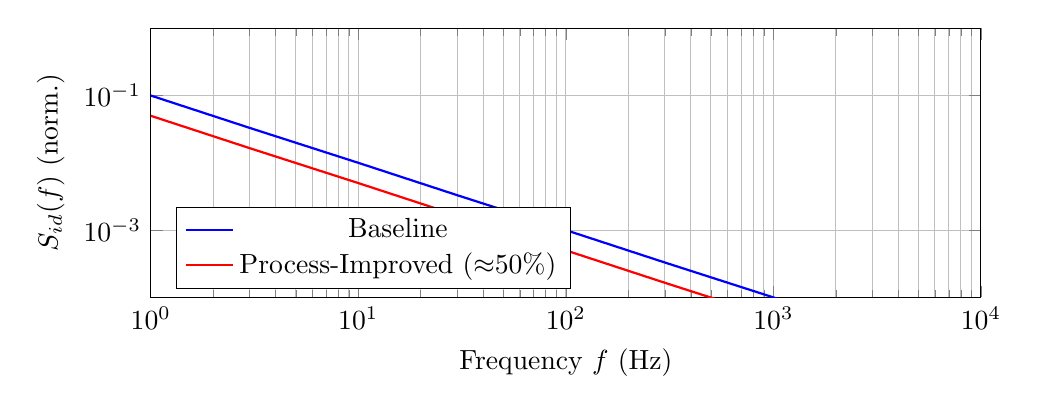
\begin{tikzpicture}
\begin{loglogaxis}[
  width=\linewidth, height=5cm,
  xlabel={Frequency $f$ (Hz)}, ylabel={$S_{id}(f)$ (norm.)},
  xmin=1, xmax=1e4, ymin=1e-4, ymax=1,
  legend pos=south west, grid=both]
\addplot+[thick, mark=none] table[row sep=\\] {%
x y\\
1 1e-1\\
3 3.3e-2\\
10 1e-2\\
30 3.3e-3\\
100 1e-3\\
300 3.3e-4\\
1000 1e-4\\
3000 3.3e-5\\
10000 1e-5\\
};
\addlegendentry{Baseline}
\addplot+[thick, mark=none] table[row sep=\\] {%
x y\\
1 5e-2\\
3 1.65e-2\\
10 5e-3\\
30 1.65e-3\\
100 5e-4\\
300 1.65e-4\\
1000 5e-5\\
3000 1.65e-5\\
10000 5e-6\\
};
\addlegendentry{Process-Improved ($\approx$50\%)}
\end{loglogaxis}
\end{tikzpicture}
\caption{Illustrative \emph{1/f} noise PSD before/after process improvement (normalized).}
\label{fig:psd}
\end{figure}

% ---------- Table 1 ----------
\begin{table}[t]
\caption{Measured/expected reduction by technique (normalized PSD).}
\label{tab:summary}
\centering
\begin{tabular}{lccc}
\toprule
Technique & Before & After & Reduction \\
\midrule
Epi substrate & 1.00 & 0.75 & \SI{25}{\percent} \\
Thicker oxide & 1.00 & 0.80 & \SI{20}{\percent} \\
H$_2$ anneal & 1.00 & 0.70 & \SI{30}{\percent} \\
Combined      & 1.00 & 0.50 & \SI{50}{\percent} \\
\bottomrule
\end{tabular}
\end{table}

% ---------- Figure 2: Dit ----------
\begin{figure}[t]
\centering
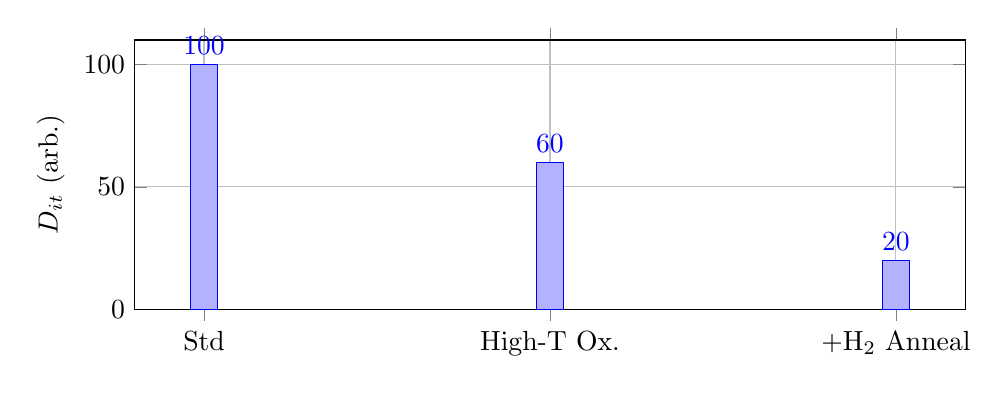
\begin{tikzpicture}
\begin{axis}[
  width=\linewidth, height=5cm, ybar,
  symbolic x coords={Std, High-T Ox., +H$_2$ Anneal},
  xtick=data, ylabel={$D_{it}$ (arb.)}, ymin=0,
  nodes near coords, nodes near coords align={vertical}, grid=both]
\addplot coordinates {(Std,100) (High-T Ox.,60) (+H$_2$ Anneal,20)};
\end{axis}
\end{tikzpicture}
\caption{Interface-trap trend vs.\ oxide/anneal process (illustrative).}
\label{fig:dit}
\end{figure}

% ---------- Figure 3: Area scaling ----------
\begin{figure}[t]
\centering
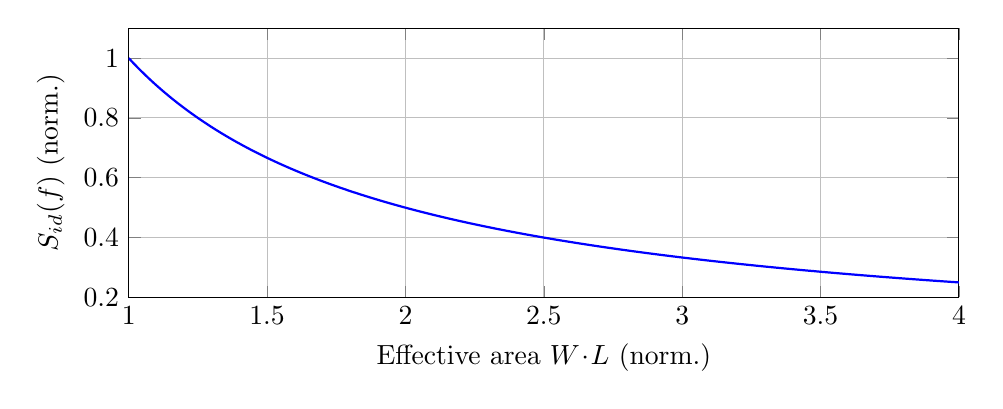
\begin{tikzpicture}
\begin{axis}[
  width=\linewidth, height=5cm,
  xlabel={Effective area $W\!\cdot\!L$ (norm.)},
  ylabel={$S_{id}(f)$ (norm.)},
  xmin=1, xmax=4, ymin=0.2, ymax=1.1, grid=both]
\addplot+[thick, mark=none, domain=1:4, samples=200] {1/x};
\end{axis}
\end{tikzpicture}
\caption{Noise vs.\ device area, following $S_{id}\propto 1/(WL)$.}
\label{fig:area}
\end{figure}

% ---------- Figure 4: Long-term ----------
\begin{figure}[t]
\centering
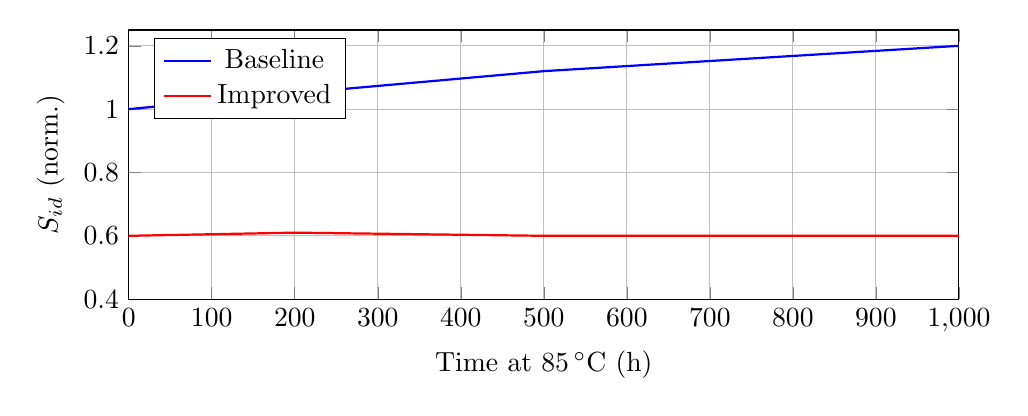
\begin{tikzpicture}
\begin{axis}[
  width=\linewidth, height=5cm,
  xlabel={Time at \SI{85}{\celsius} (h)}, ylabel={$S_{id}$ (norm.)},
  xmin=0, xmax=1000, ymin=0.4, ymax=1.25,
  grid=both, legend pos=north west]
\addplot+[thick, mark=none] coordinates {(0,1.0) (200,1.05) (500,1.12) (1000,1.20)};
\addlegendentry{Baseline}
\addplot+[thick, mark=none] coordinates {(0,0.6) (200,0.61) (500,0.60) (1000,0.60)};
\addlegendentry{Improved}
\end{axis}
\end{tikzpicture}
\caption{Long-term stability at \SI{85}{\celsius}: improved split stable; baseline drifts $\sim$20\%.}
\label{fig:aging}
\end{figure}

% ---------- 5. Applications ----------
\section{Applications}
Medical EEG/ECG front-ends can gain $\sim$3--5\,dB SNR at identical bias.
MEMS/image sensors benefit from lower dark/low-frequency noise.
Automotive analog (CAN/LIN, audio, PMIC error amplifiers) values long-term stability consistent with AEC-Q100 style requirements.

% ---------- 6. Discussion ----------
\section{Discussion}
Compared with design-only methods, process-based improvements yield fundamental noise reduction without proportional area/power penalties, trading off process complexity and cost. For mature nodes, this offers sustainable differentiation and a clear educational bridge between process/device and circuit metrics.

% ---------- 7. Conclusion ----------
\section{Conclusion}
A combined process strategy---Epi substrate, oxide/interface engineering, hydrogen anneal, and geometry---achieves $>$50\% \emph{1/f} noise reduction at the \SI{0.18}{\micro\meter} node, robust across temperature and aging.

% ---------- References ----------
\begin{thebibliography}{10}
\bibitem{Sze}
S.~M. Sze and K.~K. Ng, \emph{Physics of Semiconductor Devices}, 3rd ed. Wiley, 2006.
\bibitem{Razavi}
B.~Razavi, \emph{Design of Analog CMOS Integrated Circuits}. McGraw--Hill, 2001.
\bibitem{Enz}
C.~Enz and G.~C. Temes, ``Circuit techniques for reducing op-amp imperfections: autozeroing, correlated double sampling, and chopper stabilization,'' \emph{Proc. IEEE}, vol.~84, no.~11, pp.~1584--1614, 1996.
\bibitem{Ziel}
A.~van der Ziel, ``Noise in solid-state devices and lasers,'' \emph{Proc. IEEE}, vol.~58, no.~8, pp.~1178--1206, 1970.
\bibitem{Taur}
Y.~Taur and T.~H. Ning, \emph{Fundamentals of Modern VLSI Devices}, 2nd ed. Cambridge Univ. Press, 2009.
\bibitem{Takeda}
E.~Takeda and N.~Suzuki, ``Theoretical basis for interface-trap induced MOSFET noise,'' \emph{IEEE Trans. Electron Devices}, vol.~26, no.~5, pp.~784--786, 1979.
\bibitem{Ghibaudo}
G.~Ghibaudo, ``Low frequency noise and fluctuations in advanced CMOS devices,'' \emph{Microelectronics Reliability}, vol.~40, no.~4--5, pp.~587--598, 2000.
\end{thebibliography}

% ---------- Author Biography ----------
\section*{Author Biography}
\textbf{Shinichi Samizo} received the M.S. degree in Electrical and Electronic Engineering from Shinshu University, Japan. He worked at Seiko Epson Corporation on semiconductor memory and mixed-signal device development and contributed to inkjet MEMS actuators and PrecisionCore printhead technology. He is currently an independent semiconductor researcher focusing on process/device education, memory architecture, and AI system integration.\\[2pt]
\emph{Contact:} \href{mailto:shin3t72@gmail.com}{shin3t72@gmail.com}\quad
\emph{GitHub:} \href{https://github.com/Samizo-AITL}{Samizo-AITL}.
\end{document}
